\documentclass{TIJMUjiaoanSY}
\pagestyle{empty}


\begin{document}


%课程名称
\kecheng{Linux系统概论}
%实验名称
\shiyan{实验6\ Linux中的软件管理}
%教师姓名
\jiaoshi{伊现富}
%职称
\zhicheng{讲师}
%教学日期(格式:XXXX年XX月XX日XX时-XX时)
\riqi{2019年6月6日15:30-17:10}
%授课对象(格式:XXX系XXXX年级XX班(硕/本/专科))
\duixiang{生物医学工程学院2017级生信班(本)}
%实验人数
\renshu{28}
%实验类型
\leixing{验证型}
%实验分组
\fenzu{一人一机}
%学时数
\xueshi{2}
%教材版本
\jiaocai{Linux系统概论上机指南(自编教材)}


%教案首页
\firstHeader
\maketitle
\thispagestyle{empty}

\mudi{
\begin{itemize}
  \item 熟悉不同Linux发行版管理软件的方法。
  \item 掌握在命令行中下载文件的方法。
  \item 掌握使用APT与Yum管理软件的方法。
  \item 掌握使用dpkg与RPM管理软件的方法。
  \item 掌握通过源代码安装软件的步骤。
\end{itemize}
}

\fenpei{
\begin{itemize}
  \item (5')软件包与二进制包管理系统:回顾软件包的类型和常见的二进制包管理系统。
  \item (10')二进制包管理:回顾总结dpkg、APT和RPM、Yum管理软件的常用命令。
  \item (5')源代码安装:总结源代码安装软件的主要步骤。
  \item (5')脚本安装:总结脚本安装软件的主要步骤。
  \item (75')实验操作:以CentOS和Ubuntu发行版为例,练习Yum、RPM和APT、dpkg的使用,掌握Linux中管理软件的常用命令。
\end{itemize}
}

\cailiao{
\begin{itemize}
  \item 主要仪器:一台安装有CentOS和Ubuntu的计算机。
\end{itemize}
}

\zhongdian{
\begin{itemize}
  \item 重点难点:dpkg、APT和RPM、Yum的使用,源代码安装软件的步骤。
  \item 解决策略:通过实例进行讲解,通过演示进行学习,通过练习熟练掌握。
\end{itemize}
}

\sikao{
\begin{itemize}
  \item 列举通过命令行下载文件的常用工具,并举例说明其使用方法。
  \item Ubuntu和CentOS等常见Linux发行版使用的软件包管理系统是什么?
  \item 列举dpkg和APT软件包管理中的常用命令及其作用。
  \item 列举RPM和Yum软件包管理中的常用命令及其作用。
  \item 通过源代码安装软件的基本步骤是什么?
\end{itemize}
}

\cankao{
\begin{itemize}
  \item Linux基础及应用习题解析与实验指导(第二版),谢蓉\ 编著。中国铁道出版社,2014。
\end{itemize}
}

\firstTail


%教案续页
\newpage
\otherHeader

\noindent
\begin{enumerate}
  \item 软件包与二进制包管理系统(5分钟)
	    \vspace*{-10pt}
	\begin{multicols}{2}
    \begin{enumerate}
          \item 软件包
	\begin{enumerate}
	  \item 二进制包(预编译的软件包)
	    \begin{itemize}
	      \item deb软件包
	      \item rpm软件包
	    \end{itemize}
	  \item 源代码安装包
	  \item 脚本安装包
	\end{enumerate}
      \item 二进制包管理系统
	\begin{enumerate}
          \item dpkg及其前端APT:Ubuntu, Debian, Deepin
          \item RPM及其前端Yum:Red Hat Enterprise Linux, CentOS, Fedora
          \item ZYpp及其前端Zypper:SUSE, openSUSE
	\end{enumerate}
    \end{enumerate}
      \end{multicols}
	    \vspace*{-10pt}
  \item 二进制包管理(10分钟)
    \begin{enumerate}
      \item dpkg与APT
        \begin{enumerate}
	  \item 简介
	    \begin{itemize}
	      \item dpkg:底层工具,Debian软件包管理器的基础
	      \item APT:dpkg的前端,Debian及其派生发行版的软件包管理器
	    \end{itemize}
          \item dpkg
	    \vspace*{-10pt}
	    \begin{figure}[h]
	      \centering
	      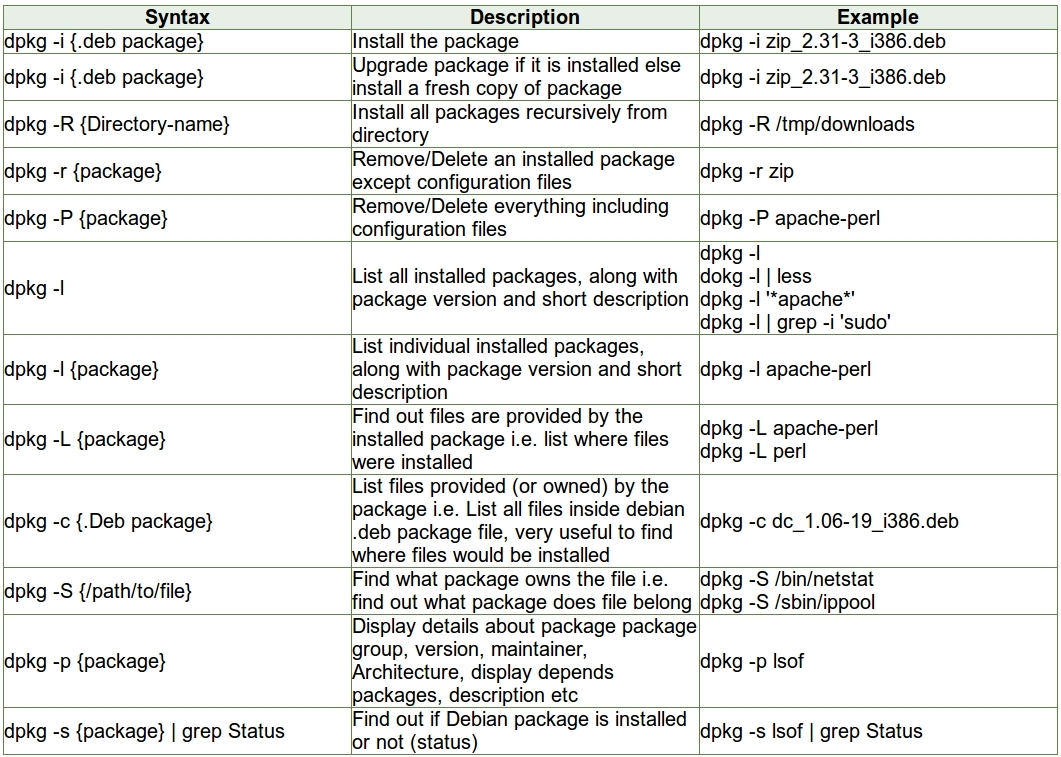
\includegraphics[width=13.5cm]{c6_dpkg_01.png}
	    \end{figure}
	    \vspace*{-10pt}
          \item APT
	    \begin{itemize}
\parpic[fr]{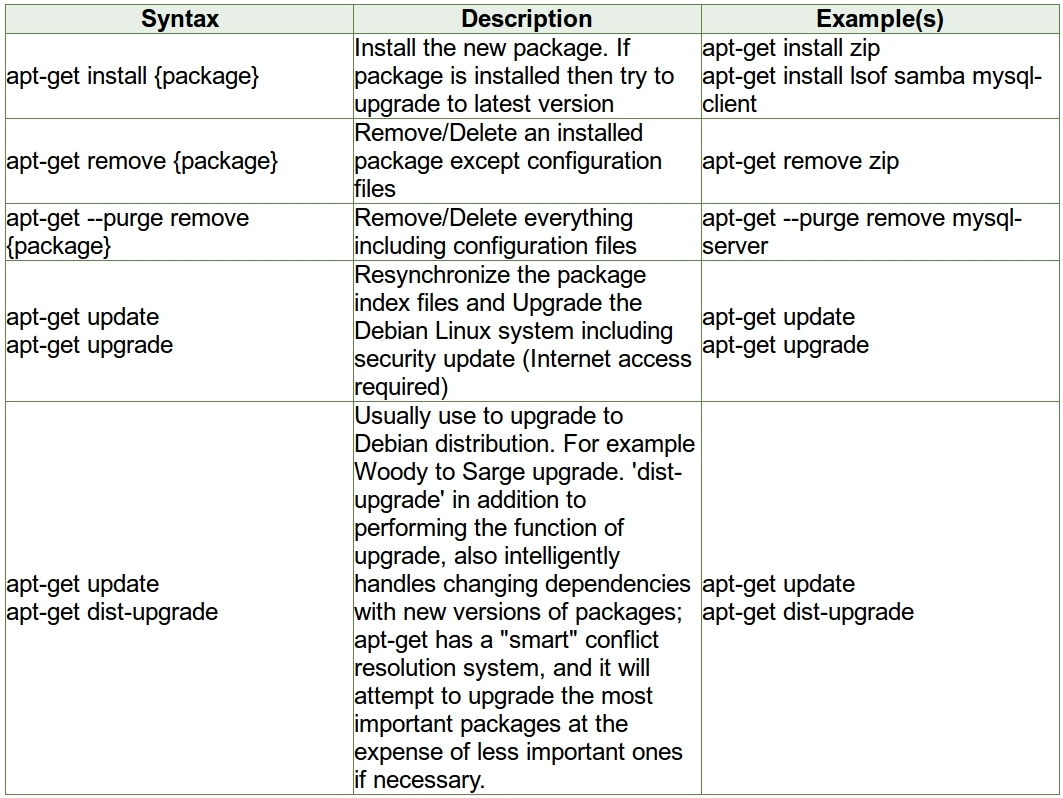
\includegraphics[width=8.3cm,height=6.2cm]{c6_apt_01.png}}
	      \item apt-get:负责软件包的在线安装与升级,底层对deb包的处理还是用的dpkg,解决依赖关系
              \item apt-cache:用来查询软件包的状态和依赖关系
              \item apt-file:负责查询软件包名称和软件包包含的文件(值得注意的是它要自己同步)
              \item apt-cross:负责为交叉编译的软件包的安装与编译等
	      \item apt-offline:可以离线安装软件包
              \item apt-build:可以简化源代码编译
            \end{itemize}
        \end{enumerate}

\otherTail
\newpage
\otherHeader

      \item RPM与Yum
        \begin{enumerate}
	  \item 简介
	    \begin{itemize}
	      \item RPM:rpm软件包管理器
	      \item Yum:RPM的前端
	    \end{itemize}
          \item RPM
	    \begin{itemize}
	    \vspace*{-10pt}
		\begin{multicols}{2}
	      \item 功能
		\begin{itemize}
		  \item 查询:-q
		  \item 校验:-V
		  \item 安装:-i
		  \item 删除:-e
		  \item 升级:-U
		\end{itemize}
	      \item 选项
		\begin{itemize}
		  \item 通用:-v
		  \item 选择:-a,-f,-p
		  \item 查询:-l,-i,-c,-d,-R,-s
		  \item 安装:-h,-\ -nodeps,-\ -prefix,-\ -test,-\ -replacepkgs,-\ -force
		\end{itemize}
	      \end{multicols}
	    \vspace*{-10pt}
	    \end{itemize}
	  \item Yum
	    \vspace*{-10pt}
	    \begin{figure}[h]
	      \centering
	      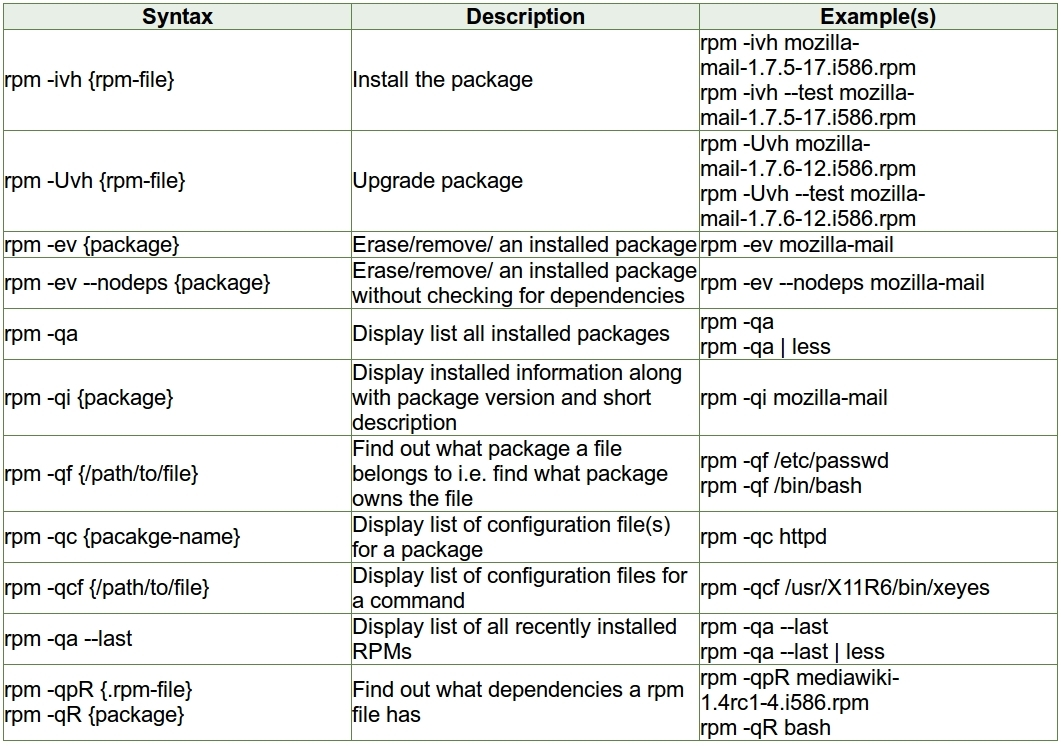
\includegraphics[width=10.5cm,height=6cm]{c6_rpm_01.png}
	      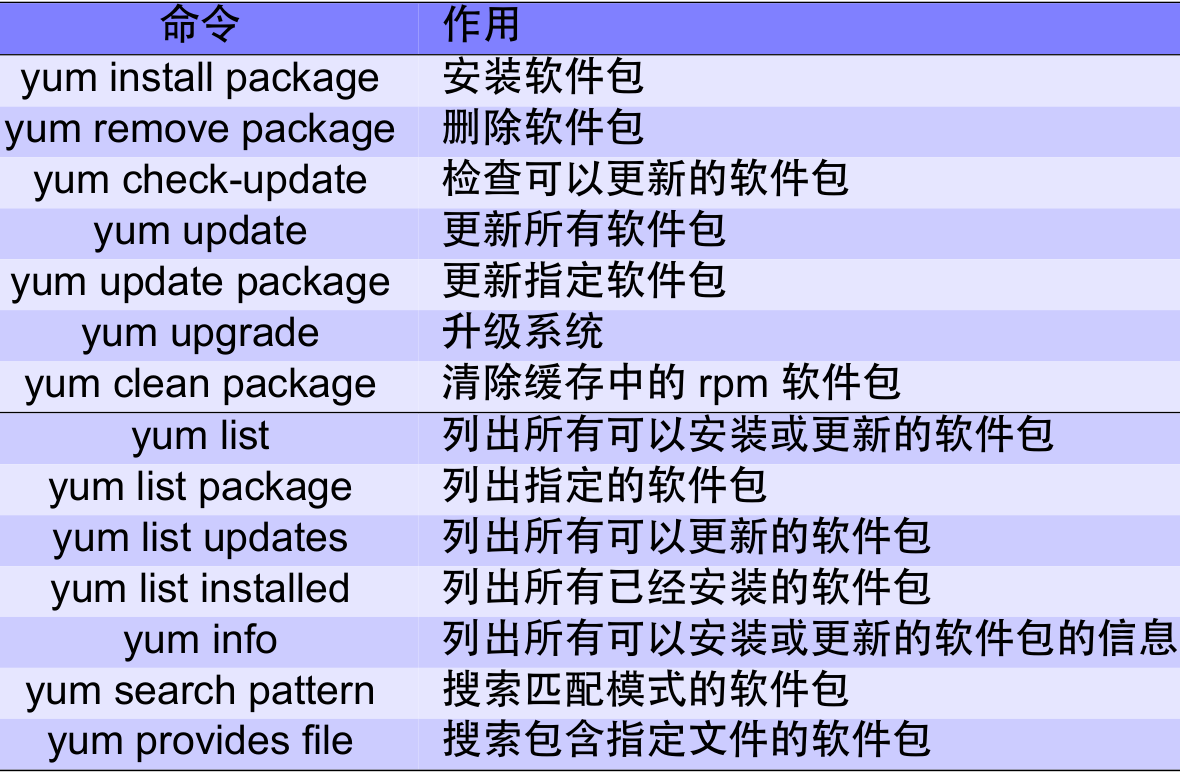
\includegraphics[width=7cm,height=6cm]{c6_yum.png}
	    \end{figure}
	    \vspace*{-10pt}
        \end{enumerate}
    \end{enumerate}

  \item 源代码安装(5分钟)
    \begin{enumerate}
      \item 准备工作
	\begin{enumerate}
          \item 下载软件:\verb|wget -c software.tar.gz|
	  \item 提取文件:\verb|tar -xzvf software.tar.gz|
	  \item 切换目录:\verb|cd software|
	\end{enumerate}
      \item 安装软件
	\begin{enumerate}
          \item 配置环境:\verb|./configure|
	  \item 编译软件:\verb|make|
	  \item 安装软件:\verb|make install|
	\end{enumerate}
      \item 其他工作
	\begin{itemize}
	  \item 阅读软件的指南或说明:\verb|vim INSTALL|,或\verb|vim README|
	  \item 指定软件的安装目录:\verb|./configure --prefix=PATH|
	  \item 安装软件前进行测试:\verb|make test|,或\verb|make check|
	  \item 以超级用户身份安装软件:\verb|sudo make install|
	  \item 删除编译产生的临时文件:\verb|make clean|
	\end{itemize}
    \end{enumerate}

  \item 脚本安装(5分钟)
    \vspace*{-10pt}
    \begin{multicols}{2}
    \begin{enumerate}
      \item 下载软件:\verb|wget -c X.tar.gz|
      \item 提取文件:\verb|tar -xzvf X.tar.gz|
      \item 切换目录:\verb|cd software|
      \item 查阅说明:\verb|vim README|
      \item 安装软件:\verb|./setup.sh|,或\verb|./install.sh|
    \end{enumerate}
    \end{multicols}
    \vspace*{-10pt}

\otherTail
\newpage
\otherHeader

  \item
    实验操作(75分钟)\textcolor{red}{(以htop、datamash、dos2unix、Glances、TeamViewer、parallel、Webmin、cheat、CPU-G等系统工具和Galaxy、FASTX-Toolkit、msort、RStudio、BEDTools、SAMtools、seqtk、WebLogo、IGV等生物信息学工具为例)}
    \begin{enumerate}
      \item 在命令行中下载软件包\textcolor{red}{(主要工具:wget,curl;主要选项:-c,-o)}
      \item 通过APT与Yum安装软件\textcolor{red}{(主要命令:apt-get install,yum install)}
      \item 通过dpkg与RPM安装软件\textcolor{red}{(主要命令:dpkg -i,rpm -ivh)}
      \item 通过源代码安装软件\textcolor{red}{(主要命令:./configure,make,make install)}
      \item 通过脚本安装软件\textcolor{red}{(主要命令:./setup.sh,python setup.py install)}
      \item 通过其他方式安装软件\textcolor{red}{(主要命令:git checkout,pip install)}
      \item 不需要安装的软件\textcolor{red}{(开箱即用)}
      \item 尝试使用dpkg与APT、RPM与Yum对软件进行管理(如:查询、安装、卸载等)
    \end{enumerate}
\end{enumerate}


\otherTail


\end{document}

